\documentclass[letterpaper]{article}

% authors and affiliations
\title{Correlated host movements can reshape spatio-temporal disease dynamics: modeling the contributions of space use to transmission risk using movement data}
\usepackage{authblk}
\author{Juan S. Vargas Soto, Lisa I. Muller, Dan Grove, Justin Kosiewska, Dailee Metts, and Mark Q. Wilber}
\affil{School of Natural Resources, University of Tennessee, Knoxville, TN}
\date{}


\usepackage[english]{babel}
\usepackage[utf8x]{inputenc}
\usepackage{amsmath}
\usepackage{graphicx}
\usepackage[left=1 in, right=1 in, top=1 in, bottom=1 in]{geometry}
\usepackage{hyperref}
\usepackage{bbold}
\usepackage{rotating}
\usepackage{bbm}
\usepackage{array}
\usepackage{xcolor}
\newcolumntype{C}[1]{>{\centering\arraybackslash}m{#1}}
% \usepackage{kbordermatrix}
\usepackage{footnote}
\makesavenoteenv{tabular}
\makesavenoteenv{table}
% \renewcommand{\theequation}{{S}\arabic{equation}}

\makeatletter
% \addto\captionsenglish{%
%   \renewcommand{\fnum@figure}{Figure S\thefigure}%
%   \renewcommand{\fnum@table}{Table S\thetable}%
% }
\makeatother

% Bibliography
\usepackage[round, colon]{natbib} % Bibliography - APA
\bibliographystyle{abbrvnat}
%\bibpunct{(}{)}{;}{a}{}{,}

% Line numbers
\usepackage{lineno}
%\def\linenumberfont{\normalfont\footnotesize\ttfamily}
%\setlength\linenumbersep{0.2 in}
\linenumbers

% Set space
\usepackage{setspace}
\doublespacing

% Command to e.g. write code that doesn't show up. Used as \ignore {some code}
\newcommand{\ignore}[1]{}

\begin{document}

\maketitle

\noindent
\textbf{Target Journal}: Ecology Letters

\section*{Abstract}

Despite decades of epidemiological theory making relatively simple assumptions about host movements, it has become increasingly clear that non-random movements and fine-scale habitat use can drastically affect disease transmission. To better predict transmission risk, theory needs to simultaneously account for how the environment affects host space use and how social dynamics affect correlation in space use among hosts. We develop new theory that decomposes the relative contributions of fine-scale space use and correlated, pairwise host movements to spatio-temporal transmission risk. Through analytical results, simulations, and application to empirical movement data, we show that even weak spatio-temporal correlations among host movements in space and time can lead to orders of magnitude differences in transmission risk at the landscape scale compared to contact and transmission metrics that only consider spatial overlap. Our theory provides clear expectations for what has been observed empirically but largely ignored in movement and disease models -- correlation in movement can reshape epidemiological landscapes, leading to hotspots of transmission whose magnitude and location are not necessarily predictable from models of joint space use.

% Understanding how animal movement influences disease transmission processes is critical to manage disease in wildlife and to eventually predict outbreaks or spillovers. These goals, however, require a thorough understanding of the intricate relationships between the environment, movement, and interactions among individuals, particularly processes with complex temporal dynamics.
% We determined how the risk of disease transmission in wildlife varies across space and time under different epidemiological conditions (parasite persistence in the environment, transmission contact distance), different degrees of social interaction, and different conditions of data availability. For this, we derived a new framework to estimate a spatially explicit, pairwise, expected risk of disease transmission based on animal movement data (e.g. GPS tracking data). We derived general conclusions related to direct transmission analytically, tested the influence of epidemiological covariates and data availability using simulations. Finally, we applied our framework to empirical tracking data of white-tailed deer. 
% We found both analytically and through simulations that temporal correlations in local space use, which arise mostly from social interactions, can significantly increase the expected force of infection (FOI), by orders of magnitude in some cases. This effect was greater for parasites with short environmental persistence (relative to host movement rate), compared to parasites with longer persistence.  
% Using empirical data from white-tailed deer, we found large differences in estimated FOI between pairs, which are not explained solely by differences in home range overlap. Individuals with more correlated movement had significantly higher FOI. These differences would scale to the population level, generating vastly different dynamics of invasion and spread.
% %Our results provide guidelines that relate the biology of parasites and the inferences that can be made regarding transmission using UDs. 
% Our approach can be easily integrated with frameworks that estimate utilization distributions accounting for environmental covariates, which would allow to create an environmentally-informed FOI that could potentially be extrapolated to other populations and locations. Understanding the environmental and social processes that generate correlations in space use will be key moving forward to accurately estimate an expected FOI  given environmental drivers. 

\section*{Introduction}

Individual movement is among the most critical factors influencing wildlife disease dynamics \citep{Dougherty2018,Manlove2022}. 
How animals move determines whether they encounter other individuals of the same species, other species, or parasites in the environment \citep{Martinez-Garcia2020,Das2023}. 
These encounters are necessary for the transmission of infectious diseases, and efforts have sought to identify where they occur, how often, and how they are influenced by environmental and social drivers \citep{Titcomb2021,Dougherty2022,Webber2023}. 
Formally linking social factors, environmental factors, animal movement, contact, and parasite transmission would improve our ability to predict and prevent outbreaks and represent a significant advancement for management of wildlife diseases.  
Nevertheless, understanding how these processes interact at an individual scale requires detailed movement information and theory to translate movement into an epidemiological context.

Most epidemiological theory is built upon the assumption of independent host movements, and there is little theory that quantifies how non-independent, correlated host movements affect contact and transmission risk. While there is a large body of empirical work that quantifies how correlated and social movements can reshape contact and transmission landscapes \citep[e.g.,][]{Kjaer2008,Grear2010,Schauber2015a}, we lack a modeling approach that isolates the role of social interactions on spatio-temporal force of infection. This limits our ability to ask questions such as: how much can correlated, non-independent movements affect spatio-temporal infection risk compared to spatial overlap? Moreover, recent studies have shown that spatial transmission risk can be highly localized \citep{Albery2021} and is not necessarily predicted by animal space use \citep{Yang2023a}. We hypothesize that non-independent animal movements can (at least partially) account for these observations and develop a modeling approach to rigorously test this hypothesis and systematically quantify the contribution of space use and correlated animal movements to spatio-temporal transmission risk.

Recent approaches developed at the interface of movement and disease ecology leverage high-resolution animal tracking data to gain insight into contact among individuals and disease transmission \citep{Richardson2015,Wilber2022,Yang2023}. For example, movement-driven modeling of spatio-temporal infection risk (MoveSTIR) builds dynamic spatio-temporal contact networks from movement data to estimate the risk of infection for different individuals across space and time \citep{Wilber2022}. MoveSTIR provides a theoretical foundation to translate contacts into the epidemiological currency of force of infection (the risk of transmission experienced by a host per unit time). These studies have highlighted the importance of individual heterogeneity and temporal scale for disease dynamics, particularly how indirect contact---individuals at the same place at different times---can significantly reshape contact and transmission networks \citep{Richardson2015,Yang2023}. Current approaches are nonetheless based on occurrence, rather than range, distributions \citep[in the terminology of ][]{Alston2022} -- meaning they only consider where animals were observed and not where they \emph{potentially} could have moved. This makes it difficult to systematically link observed encounters with environmental drivers, and to predict how social or environmental changes affect contact and transmission. 

Alternatively, spatio-temporal contact could be studied probabilistically by using utilization distributions (UDs). The UD represents the probability---transient or long-term \citep{Tao2016}---of an organism using a particular area \citep{Worton1989}. The high spatial and temporal resolution of modern tracking data serves to build UDs based on biologically realistic movement models \citep{Kranstauber2012,Fleming2014}, and to link them with underlying resources \citep{Potts2023}.
Individual UDs also serve to study pairwise interactions, for example to quantify home range overlap \citep{Winner2018}, or to estimate the expected location and rate of encounter between individuals \citep{Noonan2021}, which could be used to infer transmission risk \citep{Godfrey2010, Godfrey2013,Noonan2021}. 
Moreover, because UDs can be directly linked to environmental drivers of movement \citep{Signer2017}, they could be used for prospective analyses, to predict contact and transmission in novel environments, or to understand cascading effects of environmental and social perturbations from individual movement to population and landscape-level disease transmission. 

Current contact metrics based on UDs focus only on direct interaction, ignoring temporal dynamics that are especially relevant for epidemiological processes. The Conditional Distribution of Encounters (CDE) \citep{Noonan2021}, for example, estimates local probabilities of encounter assuming that individuals move independently from each other.
While a useful simplification, social interactions like territoriality or gregariousness can invalidate this assumption \citep{Manlove2018,Sah2018}. In these cases, temporal correlations in space use could increase or decrease the expected probability of encounter compared to an assumption of independent movement \citep{Kjaer2008,Schauber2015a}. 
Moreover, direct interactions do not necessarily equate to \emph{epidemiological contacts}, which consist of contact formation, contact duration, pathogen acquisition, pathogen shedding, and pathogen decay. As some parasites can persist in the environment for months or years (e.g. anthrax, CWD), ignoring these processes could severely underestimate transmission risk \citep{Wilber2022,Yang2023,Richardson2015}.

% The previously developed MoveSTIR implicitly accounts for such correlations, but only applies for observed data. In contrast, the CDE provides a basis for estimating encounter probabilities across the landscape, but ignores correlated movements and temporal dynamics of indirect contact.
% To assess the role correlated movement can play of epidemiological landscapes \citep[\emph{sensu}][]{Manlove2022} an approach is needed that combines the range-distribution inference of UDs and CDEs \citep{Alston2022,Noonan2021} with the epidemiological focus of MoveSTIR to link UDs with epidemiological dynamics. 

Here, we develop a model we refer to as Probabilistic MoveSTIR (PMoveSTIR) to estimate epidemiological contact and expected force of infection across space and time from UDs and correlated animal movements. We derive a general model that links transient, spatially heterogeneous UDs to transmission, and provide modifications to consider stationarity in space or time.
Deriving analytical results and applying PMoveSTIR to simulated data, we demonstrate the sometimes sizable importance of correlated host movements on pairwise transmission risk, indicating that ignoring social drivers of contact could severely bias epidemiological inference. We show that this result primarily holds for parasites with short environmental persistence (relative to host movement rate). %For parasites that persist for long periods of time in the environment, non-independent host movements are largely inconsequential compared to spatial overlap for transmission risk. 
Using a dataset of white-tail deer movements, we show that correlated movements can increase potential force of infection by orders of magnitude for a hypothetical directly transmitted parasite but are relatively unimportant for a hypothetical parasite with long persistence times. Moreover, correlated movements can yield highly heterogeneous transmission landscapes compared to spatial overlap alone, supporting the emerging idea that fine-scale patterns of transmission dynamics are common in wildlife \citep{Albery2021} and are contributed to by correlated host movements. PMoveSTIR is a key next step for developing predictive models that link movement data to spatio-temporal infection dynamics on real landscapes.

% Our approach provides probabilistic, spatio-temporal contact networks, allowing us to rigorously answer the question: how does among animal correlation shape spatio-temporal transmission dynamics?

\section*{Methods}

\subsection*{Model development - Linking utilization distributions to transmission through PMoveSTIR}

PMoveSTIR builds on the MoveSTIR model \citep{Wilber2022} and formally links utilization distributions (UDs), direct and indirect contacts, correlated animal movements, and spatial estimates of force of infection (FOI). Essentially, we want to know, for two individuals $i$ and $j$ moving and interacting across a landscape, what is the FOI $i$ experiences from $j$, across space and time?  

As in MoveSTIR, we assume that transmission happens by an infected host depositing pathogen into the environment and another host picking that pathogen up. 
Deposition and acquisition can represent a range of processes, from one individual coughing and another inhaling in a matter of seconds, to one host depositing parasite eggs or larvae in the environment and another individual consuming these days or weeks later. 
This fairly general assumption encompasses standard density-dependent transmission as a special case \citep{Cortez2021}. 
Moreover, considering transmission through deposition and acquisition clearly links direct and indirect transmission along a continuum \citep{Wilber2022}.

In PMoveSTIR, we assume ``contacts'' occur if both individuals visit a given location $x$, which could be a habitat patch or a grid cell. 
We assume that locations $x$ do not overlap so the sum of their areas equals some total area over which individuals can move (see Appendix 1 for a derivation when $x$ is a point, not an area). 
Furthermore, we assume that the likelihood of contact is uniform within the location $x$, consistent with a so-called top-hat encounter function \citep{Gurarie2013,Wilber2022}.

Given these assumptions, we define the pairwise FOI host $j$ exerts on host $i$ in location $x$ at time $t$ as \citep{Wilber2022}
\begin{equation}
    h_{i \leftarrow j}(t, x) = \int_{-\infty}^{t} \beta' \lambda \delta_{x_j(u)}(x) \delta_{I_j(u)}(I) S(t - u) du
    \label{eq:original_foi}
\end{equation}
where $\lambda$ is the pathogen deposition rate, $\delta_{x_j(u)}(x)$ is an indicator variable that is one if host $j$ is in location $x$ at time $u$ and zero otherwise, $\delta_{I_j(u)}(I)$ is an indicator function that is one if host $j$ is in an infected state at time $u$ and zero otherwise, and $S(t-u)$ is the probability that any pathogen deposited at time $u < t$ is still alive at time $t$ \citep[see][for a full derivation]{Wilber2022}. 
The term $\beta'$ is the rate at which host $i$ picks up pathogen within location $x$ and can be re-written as $\tilde{\beta} / A_x$, where $\tilde{\beta}$ can be considered a ``search efficiency'' term, with units area/time (e.g., $m^2 / day$), and $A_x$ gives the area of location $x$ (e.g., 100 $m^2$). 
Therefore, the total acquisition rate scales with the area in which contact can occur; in larger areas, the acquiring host would have to search for longer to find a ``packet'' of pathogen, reducing the total acquisition rate and the corresponding FOI. Moving forward, we assume that the depositing host is always infected. This is equivalent to building a contact network and also represents the structural form of FOI needed to compute pathogen invasion thresholds \citep{Wilber2022}.

Considering probabilistic space use (i.e., we know where an individual is at a given time and location with some probability), we can re-write equation \ref{eq:original_foi} as
\begin{equation}
    h_{i \leftarrow j}(t, x) = \int_{-\infty}^{t} \beta' \lambda \delta'_{x_i(t)}(x) \delta'_{x_j(u)}(x) S(t - u) du
    \label{eq:prob_foi}
\end{equation}
where $\delta'_{x_i(t)}(x)$ and $\delta'_{x_j(u)}(x)$ are random variables that specify whether or not (i.e., 0 or 1) host $i$ or host $j$ is in location $x$ at time $t$.  This means that $h_{i \leftarrow j}(t, x)$ is also a random variable, and we can express its expected value as 
\begin{equation}
    E[h_{i \leftarrow j}(t, x)] := h^*_{i \leftarrow j}(t, x) = \int_{-\infty}^{t} \beta' \lambda E[\delta'_{x_i(t)}(x) \delta'_{x_j(u)}(x)] S(t - u) du.
    \label{eq:expected_foi}
\end{equation}
Interpreting this expectation, we are asking: if we simulated some movement process thousands of times, what is the probability that host $i$ is in location $x$ at time $t$, and host $j$ was in location $x$ at a previous time $u$? 

\subsubsection*{Linking equation \ref{eq:expected_foi} to utilization distributions}

For two random variables $Y$ and $Z$, $E[YZ] = E[Y]E[Z] + Cov(Y, Z)$.  We can therefore write equation \ref{eq:expected_foi} as
\begin{equation}
    \begin{aligned}
        h^*_{i \leftarrow j}(t, x) &= \int_{-\infty}^{t} \frac{\tilde{\beta}}{A_x} \lambda E[\delta'_{x_i(t)}(x) \delta'_{x_j(u)}(x)] S(t - u) du \\
        &= \frac{\tilde{\beta}}{A_x} \lambda \int_{-\infty}^{t} [E[\delta'_{x_i(t)}(x)] E[\delta'_{x_j(u)}(x)] + Cov(\delta'_{x_i(t)}(x), \delta'_{x_j(u)}(x))] S(t - u) du \\
        &= \frac{\tilde{\beta}}{A_x} \lambda \int_{-\infty}^{t} [p_i(x, t) p_j(x, u) + Cov(\delta'_{x_i(t)}(x), \delta'_{x_j(u)}(x))] S(t - u) du \\
    \end{aligned}
    \label{eq:foi_cov}
\end{equation}
where we use the fact that the expectation of an indicator variable is a probability \citep{Grimmett2001}. The terms $p_i(x, t)$ and $p_j(x,u)$ give the probabilities that host $i$ and $j$ are in location $x$ at times $t$ and $u$, respectively, and can also be written as $p_i(x, t) = \int_{A_x} f_i(s, t) ds$ where $f_i(s, t)$ is the probability density of host $i$ using the point $s$ at time $t$ and the integral is over the area $A_x$ (defined equivalently for host $j$). Thus, we have obtained an equation that links the transient utilization distributions $f_i(s, t)$ and $f_j(s, u)$ with the spatio-temporal FOI.
This general PMoveSTIR formulation accounts for heterogeneity in space and time, but the model can consider other scenarios, for example when space use is uniform, or when UDs are stationary in time  (Fig. \ref{fig:square}, Appendix 2). 

For example, when UDs are stationary in time equation and pathogen decays exponentially in the environment at rate $\nu$, equation \ref{eq:foi_cov} becomes (derivation in Appendix 2)

\begin{equation}
    \begin{aligned}
    h^*_{i \leftarrow j}(x) = \beta' \lambda [ \underbrace{p_i(x)p_j(x) \frac{1}{\nu}}_{\substack{\text{FOI contribution from} \\ \text{shared space use}}} + \sigma_i(x) \sigma_j(x) \underbrace{\int_{0}^{\infty} Cor(\delta_{i \in x}, \delta_{j \in x} | s) e^{-\nu s} ds]}_{\substack{\text{FOI contribution from} \\ \text{correlated movement}}}.
    \end{aligned}
    \label{eq:stationary_cor}
\end{equation}
where $\sigma_i(x) = \sqrt{p_i(x)(1 - p_i(x))}$  and $\sigma_j(x) = \sqrt{p_j(x)(1 - p_j(x))}$ are the standard deviation in probability of host $i$ and $j$ using location $x$, respectively.  Importantly, this shows that the expected force of infection between two individuals is a result of shared space use and how correlated host movements are in location $x$ at different time lags.  The correlation term in equation \ref{eq:stationary_cor} is directly related to the probability that host $i$ is in location $x$ given host $j$ is location $x$. 
%In the upper-left corner, we consider space use is uniform, but movement is non-stationary. In this case, it is not important where an individual is, just when. Considering this framing from an empirical point of view, proximity loggers deployed on individual hosts---a commonly used tool to measure among-animal contacts \citep{Drewe2012}---only tell us when contacts between individuals occur, but not where.  Thus, we cannot make inference about spatial factors driving contacts, but can make inference on temporal processes.  We consider this case in a future study.

\subsection*{Analytical and simulation insight into correlated movement and FOI}

Leveraging PMoveSTIR, we used analytical analysis, simulation, and empirical data to ask: how much can correlated movements affect spatio-temporal infection risk for directly and indirectly transmitted parasites relative to spatial overlap? 
First, we used PMoveSTIR to derive a general formula that explicitly quantifies how much correlation can augment or reduce force of infection due to direct contact compared to random movement. We also derived analytical results for a specific movement pattern to demonstrate how correlated movements alter transmission risk due to indirect transmission.
Second, we used simulations to explore how temporally correlated movements affect  transmission, and how the pairwise FOI estimate depends on epidemiological parameters such as contact distance $d$ and parasite decay rate in the environment $\nu$. Moreover, empirically estimating the correlation component in equation \ref{eq:stationary_cor} depends amount of movement data available. Therefore, we also explored the implications of different tracking times on the estimated correlation component. For the simulations, we focused on the lower-right corner of the PMoveSTIR box (equation \ref{eq:stationary_cor}), where we assumed statistical stationarity in movement. The process for calculating the FOI across the landscape is summarized in Fig. \ref{fig:steps}.

In every simulation (we simulated 20 replicate movement tracks for each combination of parameters), two individuals moved around established home ranges according to an Ornstein-Uhlenbeck process. To create different levels of correlation, we modified the initial simulated tracks using a convolution approach with a social interaction kernel \citep{Scharf2018}. This method accounts for constant or temporally varying attraction between pairs of individuals. For our purposes we assumed attraction strength was constant in time, but varied across pairs from 0 (completely independent movement) to 1 (joint movement). Strong interactions led to similar and highly overlapping trajectories, which could represent animals in a herd, courting/mating pairs, or parents with their offspring.
For every scenario, we fitted continuous-time movement models to the simulated tracks, and estimated individual UDs using autocorrelated kernel density estimation \citep{Calabrese2016}. We estimated the UDs on a grid of square cells, where the cell side $d$ is the approximate threshold contact distance for epidemiological contact. 

We used the UDs to calculate the product of the probabilities of use ($p_i(x)p_j(x)$) and the product of their standard deviations ($\sqrt{p_i(x)(1-p_i(x))}\sqrt{p_j(x)(1-p_j(x))}$) for each grid cell. Both products are symmetrical for every pair of individuals. 
The lagged correlation term in equation \ref{eq:stationary_cor} is calculated based on the position history for each individual at locations that both visited (locations that only one or neither individual visited have a correlation of zero). This is a binary vector that specifies whether each individual was present (1) or absent (0) at location $x$ at time $t$. 
The order of visits matters, so these correlation values could be asymmetric between individuals. 
Correlations can appear spuriously even in the absence of a true interaction, particularly for time series that are autocorrelated. To address this issue, we performed a pre-whitening step to remove the potential effects of autocorrelation on the estimated cross-correlation. This procedure consists of fitting an autoregression model to one of the series, and filtering both of them using the coefficients estimated from the model \citep{Dean2016}. Additionally, we retained only correlation values that were significantly different from 0, i.e. correlations with absolute values greater than a threshold of $1.96/\sqrt(N)$, where $N$ is the length of each time series \citep{Dean2016}. All other values were set to 0 as they are considered random noise.
We then scale each correlation value by the exponential parasite survival function $S(s) = e^{-\nu s}$, where $s$ is the lag corresponding to each cross-correlation between 0 and $t-dt$, $dt$ is the (constant) time lag between observations, and $\nu$ is the death rate of the parasite in the environment. 

Substituting the terms in equation \ref{eq:stationary_cor} and scaling by the epidemiological parameters $\tilde\beta\lambda/ A_x$ we obtain the per-cell FOI. Negative correlation terms could occasionally make a cell's estimated FOI negative, especially for small cells where the probabilities of use are low (this is a statistical artifact from empirically estimating cell-level correlation); the FOI is nevertheless strictly positive by definition, so in these cases we set the cell FOI to zero.
Through these simulations we explore how the expected FOI is influenced by correlation in space use, home range overlap, parasite decay rate, and contact distance. %We also explore how the contribution from the correlation to the total and local FOI varies. 

\subsection*{Empirical application - White-tailed deer}

To test the role of space-use and correlated movements on potential transmission risk in a real system, we applied the PMoveSTIR model to GPS-tracking data for five white-tailed deer (\emph{Odocoileus virginianus}) from Ames Plantation, Tennessee, USA (one buck and four does). 
Deer were captured and equipped with GPS collars that recorded fixes every 30 minutes (Lotek LifeTrack IR 420; IACUC \# 2850-1021 from the University of Tennessee).  All individuals used in this study were captured at the end of March 2023 but we only included movement data from May to June in this study (removing April data to eliminate any capture effects on movement).  We fitted continuous-time movement models to each track and estimated the utilization distributions (UD) using AKDEs \citep{Calabrese2016}. Using the fitted continuous-time movement model for each individual, we interpolated the positions to regular 10 minute intervals to account for missed fixes \citep{Yang2023}.  We defined a contact as occurring when hosts occupied the same 10m by 10m square cell (so $d = 10$ meters). 

We modeled two hypothetical pathogens. The first pathogen had a relatively short persistence time in the environment, surviving for an average of 1 hour  ($\nu=1 h^{-1}$). In this case, transmission is largely direct and this might represent a pathogen like SARS-COV-2, which can infect and transmit between white-tailed deer \citep{Hale2022}. The second hypothetical pathogen had a long persistence time, remaining viable for over a year on average ($\nu=0.9 yr^{-1}$). In this case, transmission is largely indirect and might reflect a pathogen like chronic wasting disease (CWD), which can transmit directly and indirectly between deer and can persist for years in the environment \citep{Saunders2012a}. The $\beta$ and $\lambda$ parameters are scalars in PMoveSTIR and do not affect any relative comparisons, so we set them both to unity. As in the simulations, we pre-whitened and filtered correlation values to remove potentially spurious correlations. 
We used these data to explore how differences in overlap across home ranges and correlated movement influence the expected FOI with real animal trajectories.

\section*{Results}

\subsection*{The importance of correlated movements on FOI -- analytical results}

To gain analytical intuition into the role that correlated movement can have on FOI, consider the situation where where movement is statistically stationary and hosts use space uniformly (equation S9). 
For illustrative purposes, consider two hosts moving together across some area $A_{tot}$. We assume that 1) hosts spend $\eta$ time units within a habitat patch/grid cell before moving to the next one, 2) the pathogen survival function $S(s)$ is a step function with a survival probability of one when lag $s \leq \pi \eta$ and zero when $s > \pi \eta$.  
The term $\pi \eta$ gives the time the pathogen survives in the environment as a function of host residence time, where $\pi$ ranges from near zero for directly transmitted pathogens to some arbitrarily large number for pathogens with long environmental persistence.  
In this scenario, transmission can only occur while both animals are in the same patch. With these assumptions, we can rewrite equation equation S9 as 
\begin{equation}
    \begin{aligned}
        h^*_{i \leftarrow j}(A_x) = \beta' \lambda \left[\frac{A_x}{A_{tot}}\frac{A_x}{A_{tot}} \pi \eta + \frac{A_x}{A_{tot}}(1 - \frac{A_x}{A_{tot}}) \int_{0}^{\pi \eta} Cor(\delta_{i \in A_x}, \delta_{j \in A_x} | s) ds\right],
    \end{aligned}
    \label{eq:uniform_stationary2}
\end{equation}
recognizing that $\sigma_i(x) \sigma_j(x) = \sqrt{\frac{A_x}{A_{tot}}(1 - \frac{A_x}{A_{tot}})}\sqrt{\frac{A_x}{A_{tot}}(1 - \frac{A_x}{A_{tot}})} = \frac{A_x}{A_{tot}}(1 - \frac{A_x}{A_{tot}})$ when both hosts are using space uniformly.

\subsubsection*{Direct transmission}

For hosts that are moving together, $Cor(\delta_{i \in A_x}, \delta_{j \in A_x} | s)$ will be exactly unity when lag $s = 0$ and near unity when lag $s$ is near zero. When pathogens are strictly directly transmitted, $\pi$ is also small and if $\pi \eta << \eta$ then we can reasonably approximate $Cor(\delta_{i \in A_x}, \delta_{j \in A_x} | s) = 1$ for s from 0 to $\pi \eta$.  We can then write equation \ref{eq:uniform_stationary2} as 

\begin{equation}
    \begin{aligned}
        h^*_{i \leftarrow j}(A_x) = \beta' \lambda \pi \eta \left[\underbrace{\frac{A_x}{A_{tot}}\frac{A_x}{A_{tot}}}_{\substack{\text{Contribution due} \\  \text{to habitat overlap}}} + \underbrace{\frac{A_x}{A_{tot}}(1 - \frac{A_x}{A_{tot}})}_{\substack{\text{Contribution due} \\ \text{to correlated movement}}} \right].
    \end{aligned}
    \label{eq:uniform_direct}
\end{equation}
The relative contribution of correlation in movement with respect to the contribution due to habitat overlap is simply $(1 - (A_x / A_{tot})) / (A_x / A_{tot})=A_{tot}/A_x-1$. 
Thus, PMoveSTIR allows us to put intuitive bounds on the importance of correlated movements for direct transmission risk. 
As the area $A_x$ in which an epidemiological contact can occur gets smaller relative to the total area in which the hosts are moving $A_{tot}$, correlated movement can have an orders of magnitude larger contribution to direct transmission FOI than habitat overlap (Fig. \ref{fig:analytical_corr}). Large correlations across multiple areas add up into a significantly greater FOI across the entire landscape. 
This makes intuitive sense. If the area of potential contact is small and hosts are moving randomly, there is a very low chance that hosts will be there together at the same time. Correlated movements significantly increase this chance, even when correlation is low (e.g. 0.1). The contribution of correlation to FOI can be 10 times greater than spatial overlap if the area of contact is small (e.g., $<$ 5\% of the total area; Fig. \ref{fig:analytical_corr}).

In contrast, when $A_x$ approaches $A_{tot}$ (or more generally when the probability of using a particular area is very high), the importance of correlated movement relative to habitat overlap becomes minimal (Fig. \ref{fig:analytical_corr}). For example, if two hosts use a particular area together because of high resource availability, then it does not matter for FOI if social factors are leading to additional correlated movement. This result extends beyond epidemiological contexts and shows when correlated movements can significantly alter contact risk based on metrics such as home range overlap or CDE.

\subsubsection*{Indirect transmission}

The relative contribution of correlated movement on FOI becomes analytically more difficult to generalize for pathogens with indirect transmission. This is because the correlation function $Cor(\delta_{i \in A_x}, \delta_{j \in A_x} | s)$ can be highly non-trivial even in the simple case when two hosts are moving together. For example, even individuals that never encounter each other directly can have positive correlations at relatively short lags, and these can be greater than the correlations for individuals that do come into direct contact but only overlap partially at the same locations (Fig. S1). Determining the analytical form of $Cor(\delta_{i \in A_x}, \delta_{j \in A_x} | s)$ for common movement models is beyond the scope of this study, but we show an example with a relatively simple movement scenario in Appendix 3. The example illustrates three important points: 1) the contributions of correlated movement to indirect transmission risk depend strongly on movement dynamics as reflected in $Cor(\delta_{i \in A_x}, \delta_{j \in A_x} | s)$; 2) this contribution could potentially increase, decrease, or have no effect on local FOI depending on the lag considered; 3) the relative importance of correlations at different lags is determined by the parasite survival function.

\subsection*{Simulation study}

%The overall FOI varied more than four orders of magnitude among simulations, in response to both movement and epidemiological parameters. 
\subsubsection*{Effect of correlated movement on pairwise FOI}

In our simulations, greater interaction strengths led to higher overlap among home ranges, but there were also pairs moving independently with similarly high  ($>$0.9) overlap. %Simulations with interaction strengths greater than 0.9 all resulted in overlap values greater than 0.99, meaning the utilization distributions were always virtually identical. 
%Pairs moving independently had lower overlap values on average but also higher variance, so some pairs had similarly high overlap ($>$0.9). 
This allowed us to compare the FOI while teasing apart the effects of spatial overlap and temporal correlation in space use. 

The FOI was higher for pairs with higher interaction values (i.e. with stronger attraction), in part due to the resulting increase in spatial overlap. %This increase was due in part to higher spatial overlap, as can be seen from the higher FOI values calculated using only the stationary UD component . 
However, we saw an even greater increase in FOI when we accounted for temporal correlation, and the difference between the two increased with higher interaction strengths (Fig. \ref{fig:simresults}a). For very similar trajectories (interaction$>$0.9), the FOI with correlation was more than ten times the FOI estimated without correlation, and there was a more than 100-fold difference for perfectly overlapping trajectories.  

% Methods that ignore temporal correlation could therefore be significantly underestimating transmission risk. 

The FOI was generally greater when we accounted for correlation; in only 19\% of cases the estimates were equal with or without correlation, and in no instance was there a decrease. This is to be expected as we only included attraction in the simulations. 
We found that correlation could increase the estimated FOI even for pairs that moved independently. While this was generally rare (86\% of cases had less than 20\% increase), % In 75\% of these simulations there was virtually no difference in FOI estimates with and without correlation, and 86\% saw less than 20\% increase. 
there were  instances where the estimated FOI was more than three times greater. This was more likely for pairs with a high degree of home range overlap (Fig. \ref{fig:simresults}d). 
%For pairs with low overlap, on the other hand, correlation usually did not play a significant role. % Mark here:  Here is what I struggle with for this result.  If the "truth" is no correlation (which we simulated), how do we get correlation?  To me this seems like it must be Type I error.  We are testing thousands of points for correlation and, by chance alone, we are going to **statistically** pick up correlation even if none actually exists.  One way to deal with this would be to use a bonferonni correction and set all correlation values that aren't "significant" after the Bonferronni correction to 0.  This removes a lot of those spurious correlations. 
% JUAN: Yes, most correlation values are just noise. We can remove them just by using a standard threshold that depends on the length of the series. There is still an issue that I think is due to the number of visits per cell. When there are few visits by one of the individuals (<~5), that's when you get the highest correlation values (relative to the cell's expected encounter rate). These values are high enough to be considered significant. For the same pair, with more points you get lower cumulative correlations. I tested this with the empirical data, but haven't tried to include it in the simulations.  	
While the expected correlation is 0 when individuals move independently, joint space use could lead to apparent correlations, especially when there are few observations in a given cell. Apparent correlations can occur even after pre-whitening and removing the majority of statistically spurious correlations. This is important to consider when analyzing empirical data where the true correlation and the degree of attraction/avoidance among individuals are unknown. Temporal reshuffling methods such as those proposed by \cite{Spiegel2016} can be a useful tool to establish the baseline ``apparent'' correlations that appear for non-socially interacting individuals.

\subsubsection*{Influence of epidemiological parameters}

%We also analyzed how changes in epidemiological parameters, namely the parasite decay rate and the contact distance, influenced the estimated risk of transmission. 
The FOI was inversely proportional to decay rate, meaning the risk of transmission is greater for parasites that can survive longer in the environment, all else being equal (Fig. \ref{fig:simresults}b). %This effect is driven mostly by the linear increase in the spatial overlap component ($p_i(x)p_j(x)/\nu$), for longer decay times the relative contribution of the correlation term decreased significantly (Fig. \ref{fig:simresults}e). 
However, the increase in FOI due to correlated movement is greatest for parasites with short survival times. While longer parasite survival times increase the probability of indirect epidemiological contact, the expected rate of encounter at longer lags approximates the expected rate of encounter under independent movement, so correlations at long lags have only a small modifying effect on the expected FOI (Fig. \ref{fig:simresults}e). 

While FOI generally increased as decay rate decreased, longer contact distances could increase or decrease FOI, depending on interaction strength. %For pairs with low interaction strength there was no noticeable effect of increasing the threshold contact distance 
(Fig. \ref{fig:simresults}c). %However, for similar trajectories (interaction $>$ 0.9), FOI increased between two and five-fold as contact distance increased, while for identical trajectories (interaction = 1) FOI decreased. 
%In our simulations, longer threshold distances translate to larger grid cells, where the risk gets diluted. 
These changes in overall FOI respond to the effect of correlation. Increasing the contact distance increases the probability of finding two individuals in the same cell, and would therefore increase the relative contribution of correlation most for trajectories that are already close in space and time (Fig. \ref{fig:simresults}f), while it would have no effect for trajectories that are far from each other. For identical trajectories, however, grouping observations into larger cells imply fewer cells where correlation is impacting the FOI, and can thus reduce the cumulative contribution of correlation and overall FOI. 


\subsubsection*{Influence of data availability}
%The length of the data series had a significant influence on estimated FOI. 
With longer time series, the number of cells that both animals visited, and for which correlation is calculated, increased linearly. As a result, we estimated greater overall FOIs (although the local correlation values could decrease) when there was more tracking data (Fig. \ref{fig:simresults}e). 
%However, the proportion of those cells where the FOI estimates were different with and without the correlation component actually decreased. This could be interpreted as a decrease in the estimated correlations as more visits are made to the same cells. 
%While the proportion of cells that effectively modify the FOI decreases, the absolute number of these cells is still greater, and the overall effect is an increased FOI when there are longer time series. 
Since we did not include any environmental drivers of movement, the expected correlation is uniform across the landscape. The cumulative correlation, however, is not related to the product of the UDs or the product of the standard deviations. [Juan, could we add a a bit more on why this result matters?]
%Getting more data means that the correlations at the local (cell) level become more accurate, and that the correlation can be estimated for more locations. %Empirical movement studies should therefore try to ensure that the tracking duration is sufficient for the animals to cover the majority of their home range, so that estimated correlations are representative of the true underlying relationship. Given the complexity of the correlation, which may be determined through a combination of environmental factors and specific social interactions, predicting the underlying correlation surface could prove quite challenging. 


\subsection*{Empirical example: white-tailed deer}

The total potential FOI varied more than six orders of magnitude across pairs of deer, partially due to the difference in spatial overlap, which ranged between 0 and 90\% (Bhattacharyya coefficient; Fig. \ref{fig:empiricalres}). While higher overlap generally correlated with higher FOIs, we estimated significantly higher values when we accounted for correlation in movement, and the difference was not necessarily related with greater overlap (Fig. \ref{fig:empiricalres}a-c).  For the pair with the highest spatial overlap, the FOI was more than ten times greater when we accounted for correlation. Temporally reshuffling the trajectories of these individuals following \cite{Spiegel2016} confirmed that this increase in FOI due to correlation was far beyond what we would expect from any  spurious, ``apparent'' correlations that could arise in independently moving hosts (as identified in our simulations). For all pairs considered, ignoring correlation could result in between 5\% and 96\% underestimation of FOI. These effects of correlation on FOI were strongest for pathogens with a fast decay rate. For a parasite like CWD that can persist for very long in the environment, the FOI was virtually identical with or without correlation in host movement (Fig. \ref{fig:empiricalres}c). 

Given the localized nature of interactions, the changes in overall FOI are caused by increases at particular cells. Consequently, the estimated FOI is heterogeneous across the landscape (Fig.\ref{fig:empiricalres}b). These effects at the local and individual scale affect population-level parasite transmission. For example, given a simple Susceptible-Infected-Recovered model, the $R_0$ on our network of five individuals was more than ten times greater when we accounted for correlation (Fig. \ref{fig:empiricalres}d). Thus, we would expect more explosive transmission through a network that considers fine-scale space use and correlation compared to one that assumes fine-scale space use and independent movement.

\section*{Discussion}

We develop a new model PMoveSTIR that disentangles the contributions of spatial overlap and correlated movements to spatio-temporal contact and transmission risk.  PMoveSTIR explicitly emphasizes processes relevant for transmission, such as contact---direct and indirect---among individuals, parasite shedding and survival in the environment, and, importantly, correlation in space use. 
This framing sets our model apart from recent developments for inferring contact, which focus only on direct encounters and assume hosts move independently \citep{Noonan2021,Das2023}.  In particular, assuming independent host movement can significantly underestimate transmission risk, with consequences for inferred disease spread across the population. Our results provide clear expectations for what has been previously observed empirically but largely ignored in movement and disease models -- correlation in movement can reshape epidemiological landscapes, leading to hotspots of transmission whose magnitude and location are not necessarily predictable from models of joint space use.

PMoveSTIR provides a clear, quantitative guide to assess when fine-scale, temporally synchronous movement data are necessary for capturing disease dynamics and when coarser scale, asynchronous data focused strictly on UD estimation and fine-scale habitat use can be sufficient. 
In particular, we show that correlation in movement and synchronicity can be critical aspects of transmission for faster-paced parasites, i.e. parasites with short environmental persistence and transmission driven by short-term contacts \citep[cf.][]{Dougherty2018,Manlove2022}, such as canine distemper virus, rabies, \emph{Mycoplasma ovipneumoniae}, or SARS-COV-2 (SCV2). 
SCV2 is of particular public health interest and recent studies have shown that it can infect a wide-range of wildlife hosts, including white-tailed deer \citep{Palmer2021,Hale2022}. There is also evidence that white-tailed deer can transmit SCV2 between each other in controlled experiments and in the wild \citep{Martins2022,Hale2022}, suggesting SCV2 can successfully invade, spread, and persist in wildlife.  In our analysis of empirical white-tailed deer movements, we found that ignoring correlation in movements and focusing only on patterns of space use led to a ten-fold change in $R_0$ for a SCV2-like pathogen on even a simple network, with significant implications for pathogen spread.  In contrast, our simulation and empirical results show that correlation may only have marginal effects on transmission of parasites with longer persistence times like chronic wasting disease (CWD) and anthrax, and joint space use would be largely sufficient for understanding local transmission risk.


% Interestingly, transmission patterns of CWD in white-tailed deer only partially support this finding, as increased genetic relatedness (a proxy for social connectedness) increased the probability of infection beyond shared space use \citep{Grear2010}. Given the complex relationship between animal movements and time-lagged correlations (Fig. S1), there could be scenarios where correlations or direct contacts can disproportionately affect transmission risk even for pathogens with long environmental persistence.  PMoveSTIR provides a theoretical foundation to explore these scenarios in future studies.

Correlations in space use that are not accounted for by UDs typically reflect social interactions, for example
herding animals, parents with their offspring, or mates temporally moving together \citep{Scharf2016,Yang2021}. 
White-tailed deer female groups, for example, have high social affinity, especially during gestation and rut \citep{Koen2017}. Thus, pairs of deer with equivalent habitat overlap have substantially higher contact rates when both individuals are within the same social group \citep{Schauber2007a,Kjaer2008,Schauber2015a,Grear2010}. This is likely the case in our empirical study; the pair with the greatest home range overlap and potential FOI were does, almost certainly from the same group. The potential FOI was over 10 times greater than for other pairs, despite similar degrees of habitat overlap. Importantly, 91\% of the total FOI (for a hypothetical directly transmitted pathogen like SCV2) would be missed if we only considered overlapping UDs for these individuals \citep[e.g., using a metric like CDE][]{Noonan2021}. While the importance of social interactions for contact rates has been documented previously in white-tailed deer \citep{Grear2010,Schauber2015a}, PMoveSTIR allows us to directly quantify the contribution of these social interactions to the FOI and move from qualitative conclusions to movement-informed quantitative models of disease invasion.

In practice, however, correlations influencing FOI may arise from fine-scale temporal patterns of resource use unrelated to social interactions. For instance, consider two individuals independently visiting a common resource at similar times \citep[e.g., a watering hole,][]{VanderWaal2017}. If the resource is highly localized in space and time, the joint, stationary UD would not necessarily predict this as an area of high contact and transmission risk. Rather, observed contacts in this area would be associated with correlation in movement and not long-term, predicted space use.
Alternatively, temporally varying UDs (i.e., the top right corner in Fig. \ref{fig:square}) would correctly capture that the joint occurrences were a result of spatio-temporal patterns of space use, reducing the relative importance of correlations on FOI. Unfortunately, non-parametrically estimating transient UDs at fine temporal scales with limited data points is not often feasible. Therefore, while the correlation term of PMoveSTIR will remain crucial to capture epidemiologically important spatial correlations in movement, it does not always provide an exact separation between spatial and social factors driving transmission risk.

A key challenge associated with PMoveSTIR is empirically estimating the correlation surface.  While this term is well-defined in theory (equation \ref{eq:stationary_cor}), estimating fine-scale correlations from finite animal movement data without some type of spatial interpolation will inherently provide a patchy view of the true correlation surface (e.g., Fig. \ref{fig:steps}).  Our simulations showed that when animals were experiencing known social attraction at a time lag of zero, empirically estimated spatial correlations without spatial interpolation always underestimated the contribution of correlation to FOI. This is not surprising because without interpolation we are limited to analyzing spatial correlations where joint occurrences were observed and not where they potentially could have occurred. While there are tools available for spatial interpolation (e.g., Kriging from a spatially-explicit statistical model, Clough-Tocher 2D interpolators, etc.), we did not consider these here because we sought to provide a conservative view of how correlation could reshape epidemiological landscapes.  However, to adequately predict transmission landscapes out-of-sample, future work will need to develop robust approaches for estimating and predicting the entire correlation surface (some suggestions and examples in Appendix X). 

By linking movement data and inferred contact with underlying environmental factors, a broad goal of PMoveSTIR is to create an epidemiological risk landscape independent of geographical location \citep{Manlove2022}. This landscape could enable out-of-sample prediction of transmission risk, for example to forecast future disease dynamics in the study population, project population-wide disease spread as information on more individuals becomes available, or quantify transmission risk for other populations in similar environments. Previous studies have created system-specific models that make this link, for example using probabilities of use informed by step selection functions with environmental covariates to simulate local disease dynamics \citep{Merkle2018}. Our model provides a generalizable theoretical foundation to perform similar analyses across different host-parasite systems, and it can be integrated with any UD estimation method \citep{Signer2017,Merkle2018,Michelot2020,Potts2023}. In addition to movement covariates, PMoveSTIR can also incorporate spatially and temporally heterogeneous epidemiological parameters, for example parasite survival rates that vary between habitats and seasons \citep{Daversa2017}, or spatially localized shedding \citep{Weinstein2018a}. 

Predicting epidemiological landscapes from host movements relies on the key assumption that environmental characteristics strongly influence movement and space use. While there is a growing number of methods that quantify the effect of environmental characteristics on movement and habitat use \citep[reviewed in][]{Hooten2017a}, there has been much less work exploring how (and if) environment affects and predicts correlation and synchrony among hosts.  Therefore, an essential next-step for building epidemiological landscapes will be predictive models of spatio-temporal correlation among individuals.  This is an open challenge, though recent progress in predicting the dynamics of group formation will likely be key \citep[e.g.][]{Brandell2021}.
Our analyses emphasize the importance of this next step by showing that correlations at a local (cell) scale can create a vastly more heterogeneous transmission landscape, where adjacent cells could have widely different risks of infection.  Moreover, correlations can lead to localized transmission hotspots that are not necessarily predictable from joint space use \citep{Yang2023a}, and may contribute to the growing empirical recognition that fine-scale, localized transmission hotspots are present in many empirical host-parasite systems \citep{Albery2021}.  Whether these localized transmission hotspots are predictable \emph{a priori} remains to be seen, but ignoring correlated movements can make the task orders of magnitude more difficult for some pathogens.

\clearpage


\begin{figure}
    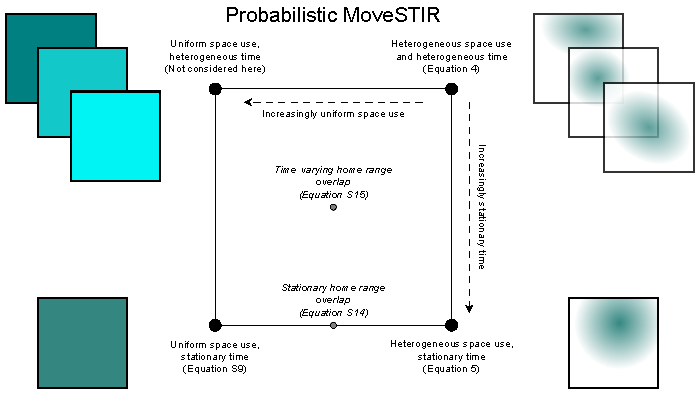
\includegraphics[width=\textwidth]{figures/conceptual_figure_pmovestir_mod.pdf}
    \caption{Conceptual figure describing the model developed in this manuscript: probabilistic movement-driven modeling of spatio-temporal infection risk. PMoveSTIR can be thought of as square where the dimensions represent heterogeneity in space and time. The upper right-hand corner is the most general case: heterogeneous space use by hosts, and movement dynamics that are not statistically stationary.  As space becomes increasingly uniform or movement becomes more statistically stationary, PMoveSTIR reduces to the upper-left hand corner or the lower-right hand corner, respectively.  We primarily focus on the lower-right hand corner in this manuscript.  When space use is uniform and movement is statistically stationary, we are in the lower-left hand corner and recover mass action transmission as a special case (Appendix 2; assuming host movements are uncorrelated).}
	\label{fig:square}
\end{figure}

 \begin{figure}
     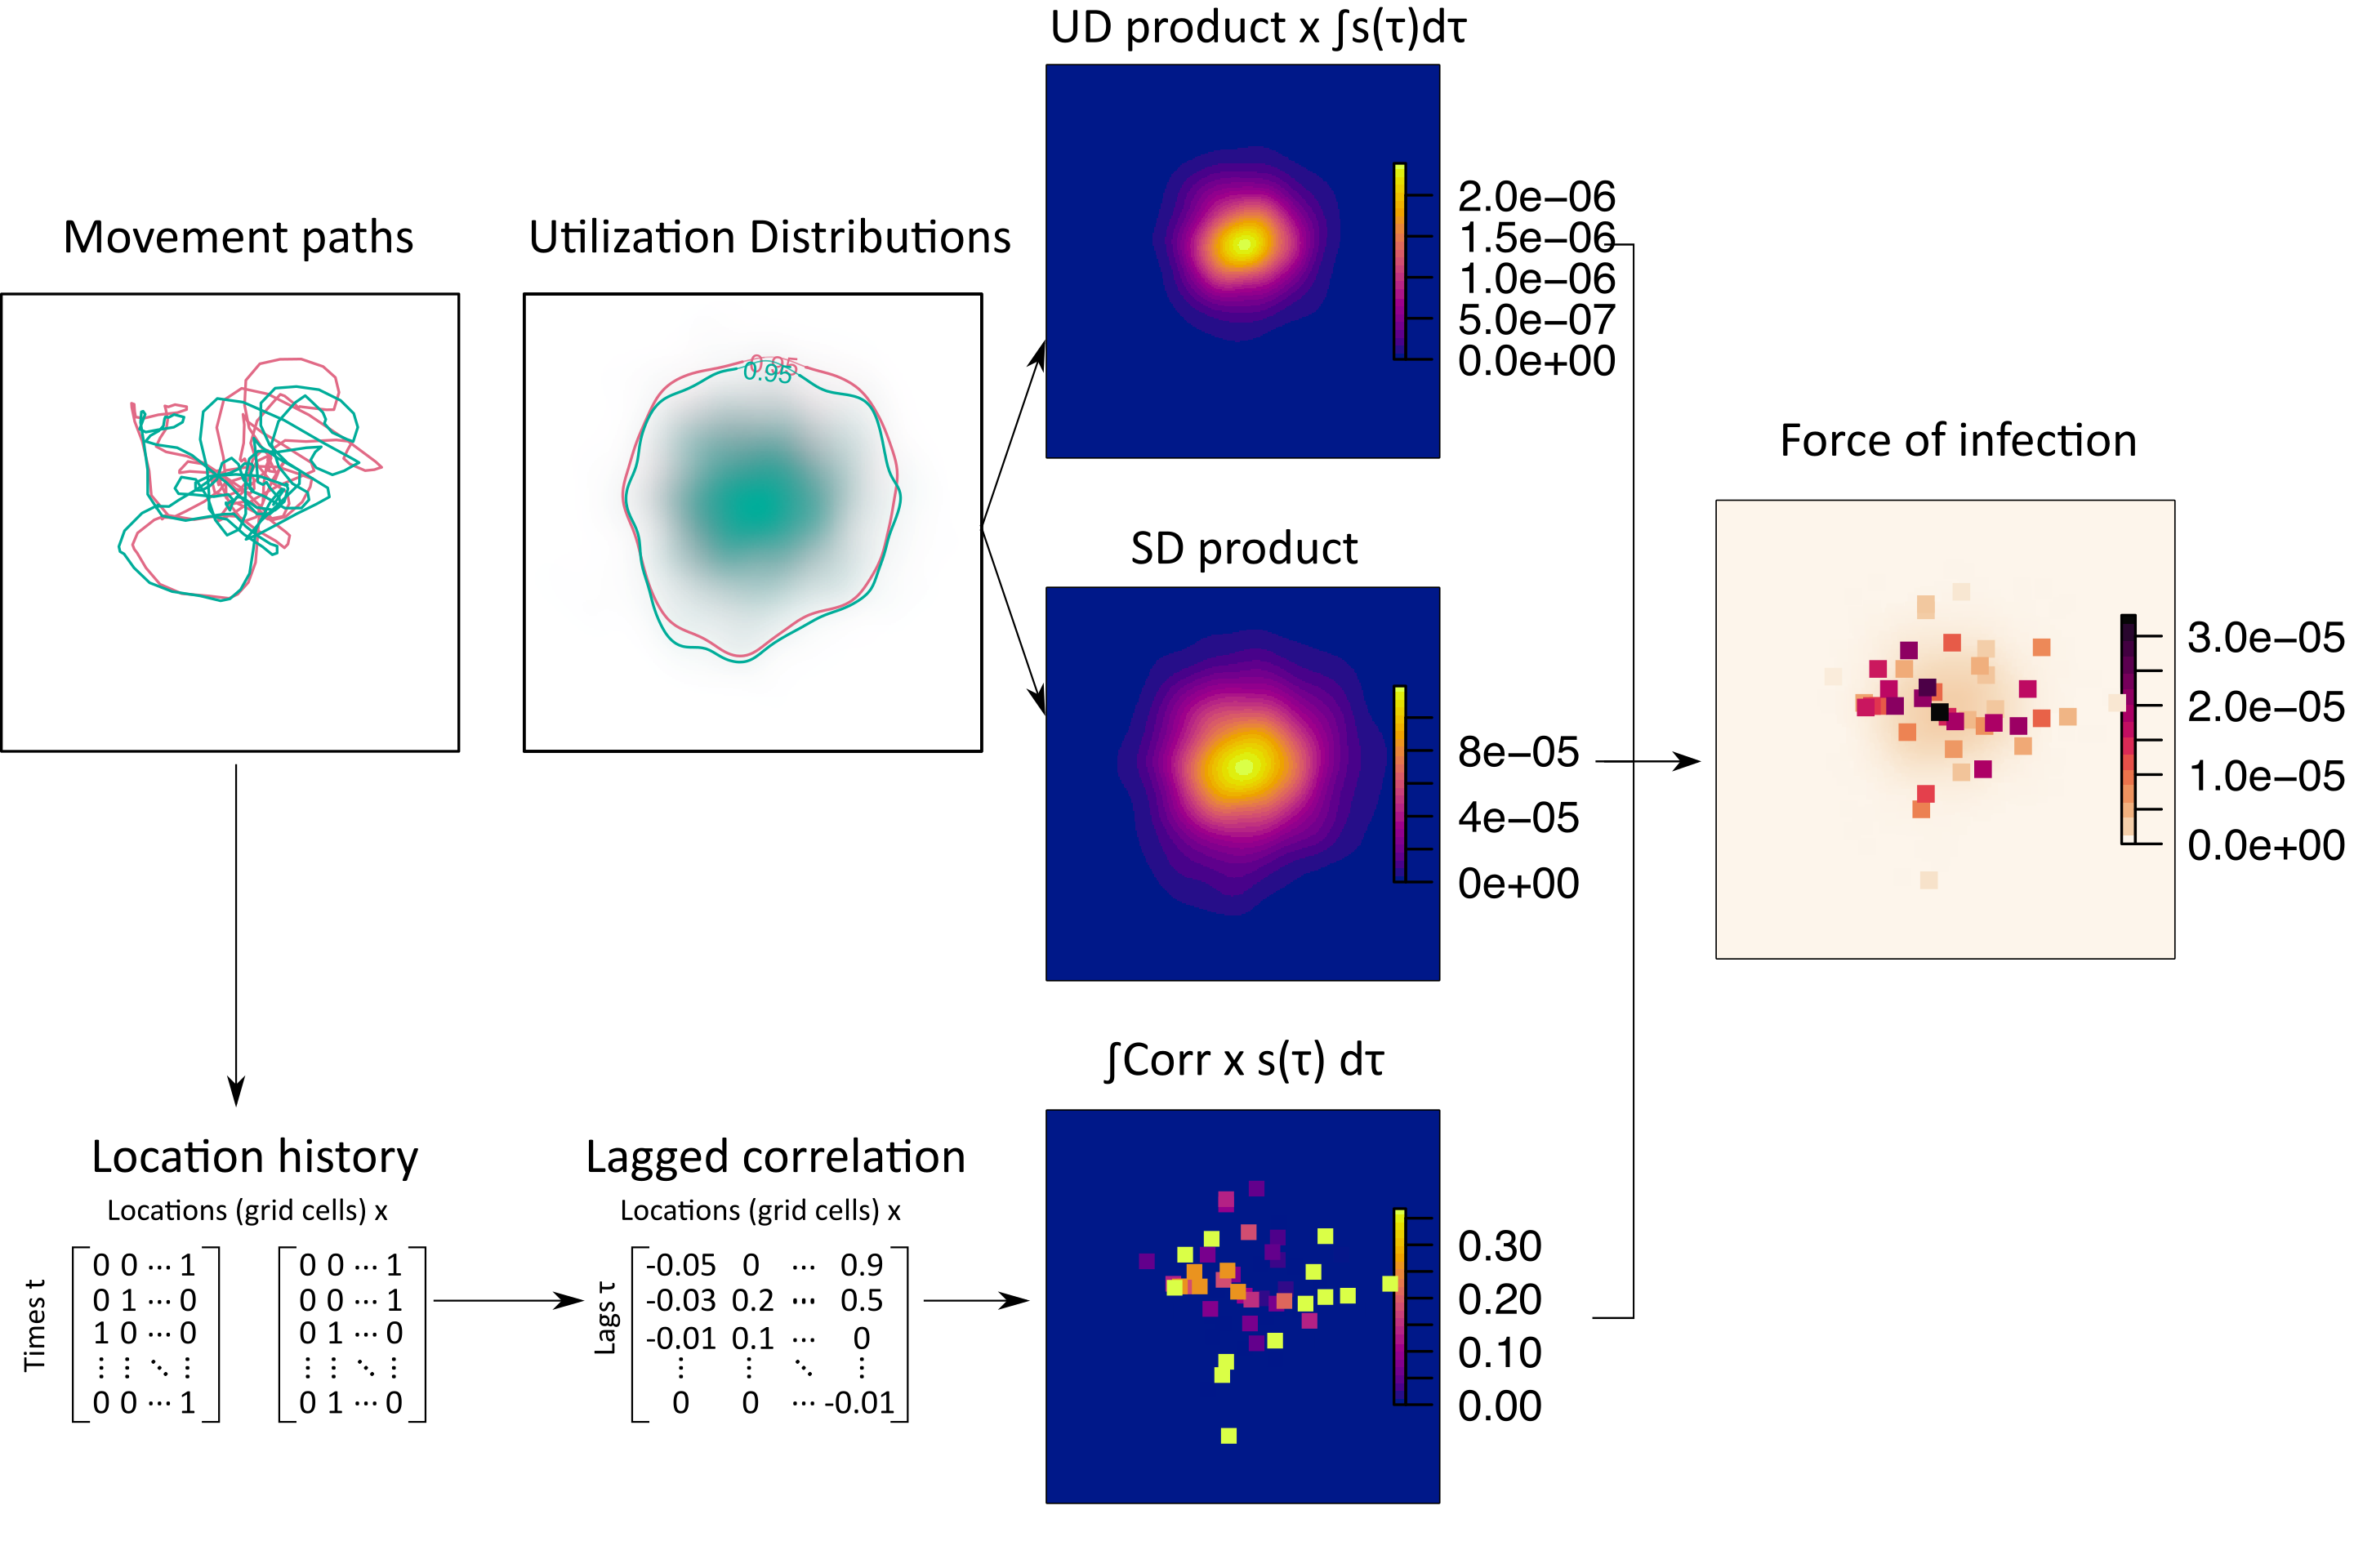
\includegraphics[width=\textwidth]{figures/steps_diagram.png}
     \caption{Flow diagram for calculating spatial force of infection (FOI) from movement data using PMoveSTIR. Starting from position data, we estimate individual utilization distributions, and use them to estimate the product of the UDs and their standard deviations (SDs). In addition, individual position histories are used to estimate the pairwise temporal cross-correlation in space use at each cell (e.g., the correlation term in equation \ref{eq:stationary_cor}). All three elements are combined and scaled by epidemiological parameters to obtain a spatially explicit, pairwise, directional FOI. Note that here and in the manuscript we do not spatially interpolate the correlation surface. We therefore provide a conservative view of how correlation contributes to landscape level FOI. For an an example of spatial interpolation of the correlation surface, see Appendix X.}
 	\label{fig:steps}
 \end{figure}

\begin{figure}
    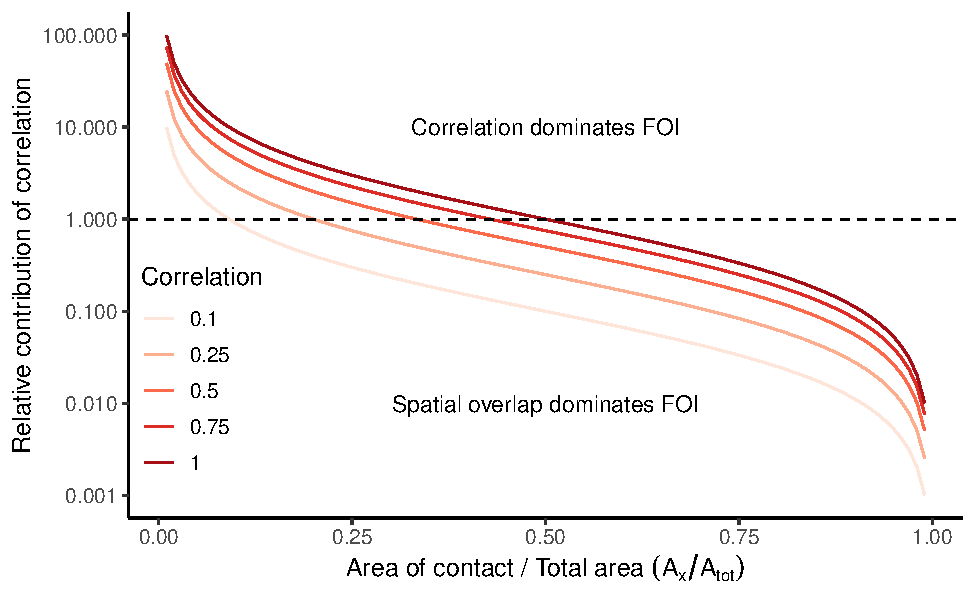
\includegraphics[width=\textwidth]{figures/correlation_analytical_figure.pdf}
    \caption{The relationship between the relative contribution of correlation in movement and spatial to pairwise force of infection (FOI) and the relative area of contact. This analytical relationship is derived in equation \ref{eq:uniform_direct} assuming direct contact.  When the relative area of contact is small relative to the total area over which animals can move (e.g., $<$ 10\%), even weakly correlated movements can significantly increase force of infection relative to spatial overlap.}
    \label{fig:analytical_corr}
\end{figure}

\begin{figure}
    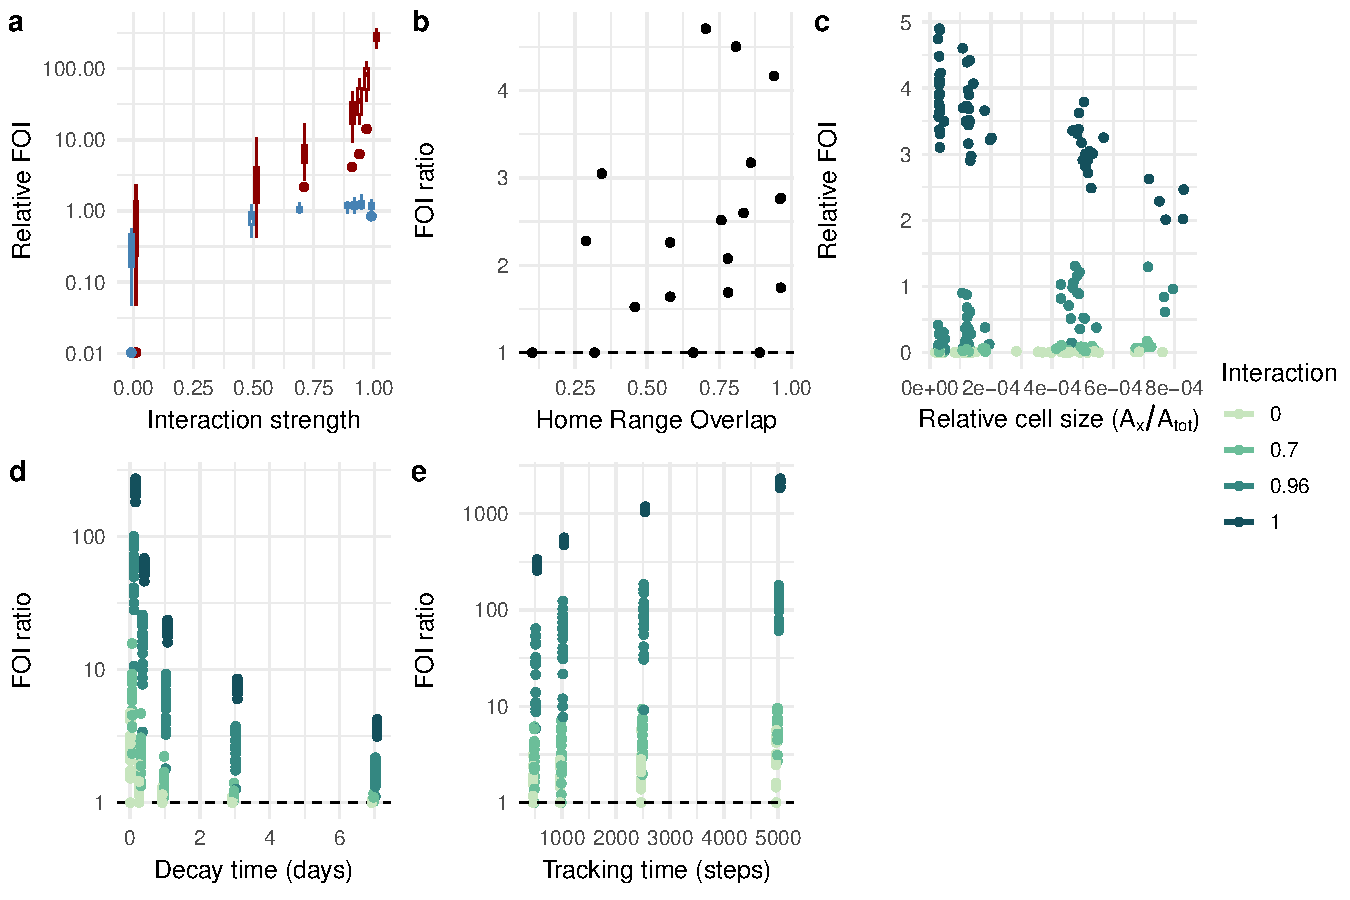
\includegraphics[width=\textwidth]{figures/sim_results.pdf}
    \caption{Analysis of simulated movement data show how the force of infection (FOI) varies depending on strength of attraction between individuals and epidemiological parameters such as the pathogen decay rate, the threshold distance that defines a contact, and the data availability.  \textbf{a)} FOI generally increases as a function of attraction strength, but the estimated values are greater when correlation is considered (red boxplots) than when only spatial overlap is considered (blue);  \textbf{b)} The estimated FOI as a function of home range overlap (as measured by the Bhattacharyya coefficient) shows how correlation can have an apparent effect even for animals that move independently;   \textbf{c)} Longer epidemiological contact distances can increase, or have no effect on the estimated FOI, depending on the interaction strength; \textbf{d)} The contribution of correlation to the overall FOI decreased with longer decay times; \textbf{e)} The FOI ratio increases with longer time series as correlation information becomes available for a larger proportion of the space used. A FOI ratio greater than one indicates that correlated movement is increasing FOI relative to spatial overlap and a ratio less than one indicates that correlated movement is decreasing the FOI. In c-e, darker shades indicate stronger attraction between individuals. }
	\label{fig:simresults}
\end{figure}

\begin{figure}
     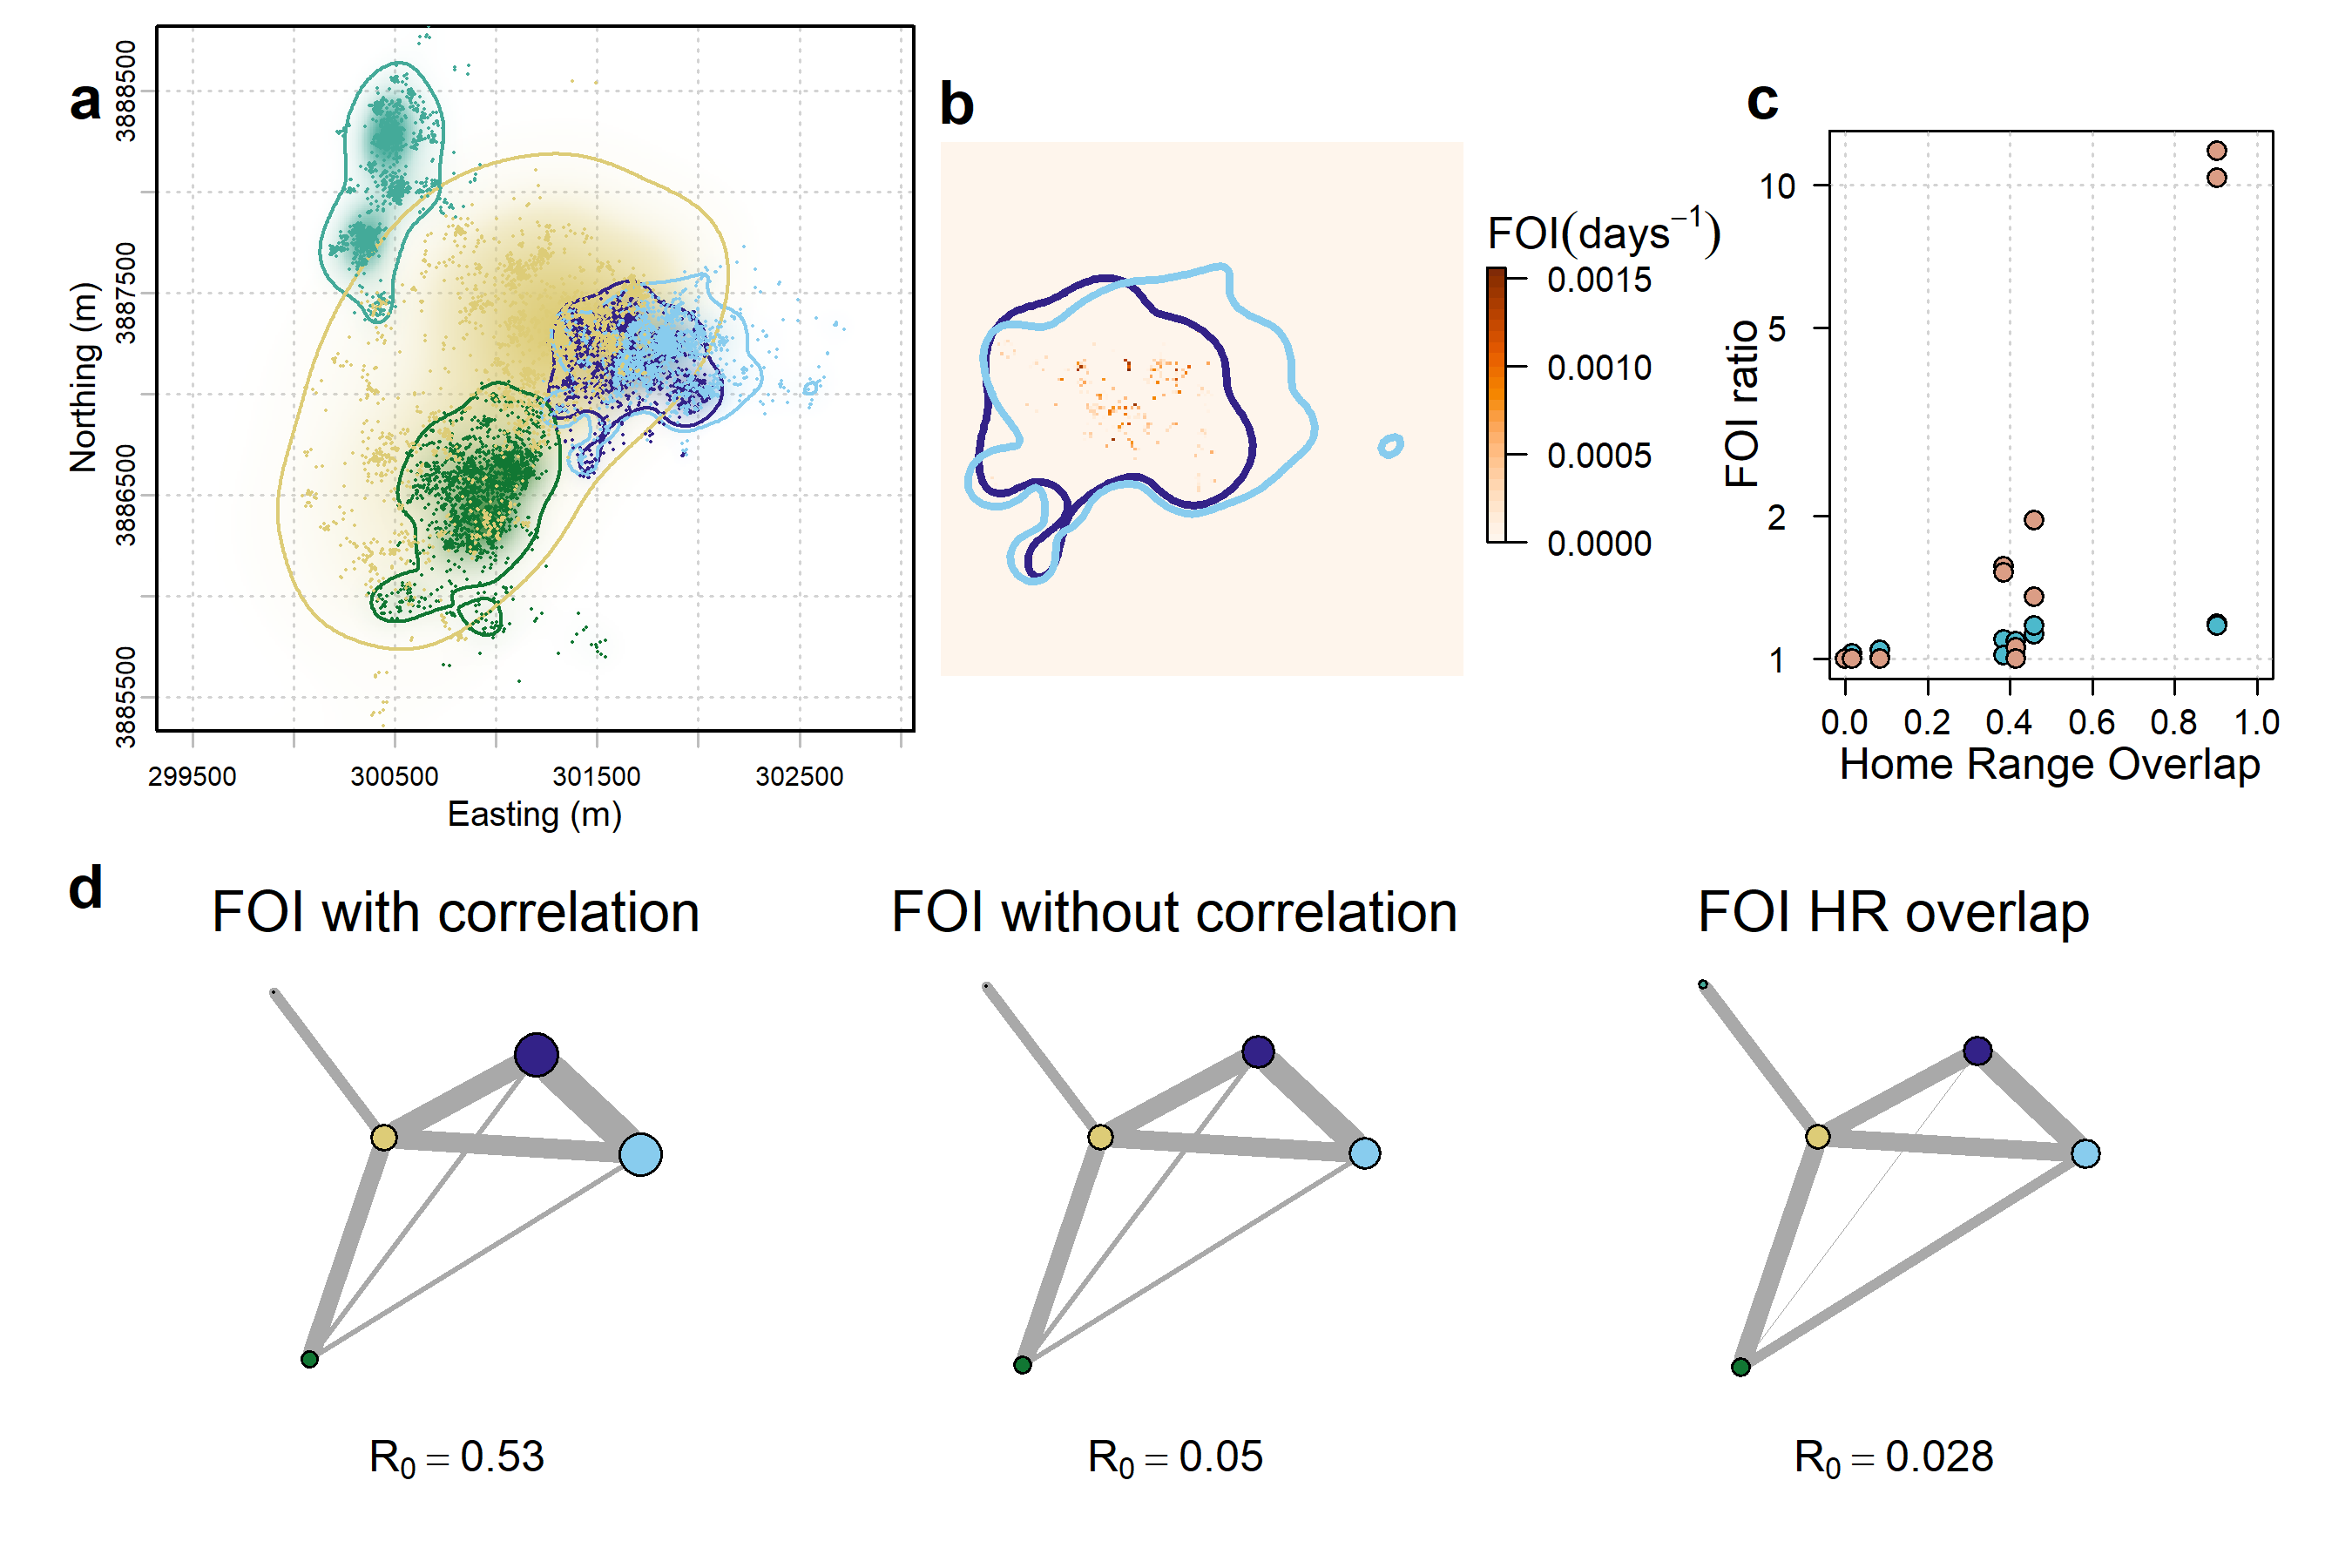
\includegraphics[width=\textwidth]{figures/deer_results.png}
    \caption{Application of the PMoveSTIR framework to movements of white-tailed deer in TN, USA. \textbf{a)} Home ranges of five individuals with different degrees of overlap. The points show the GPS locations, and the lines are the boundaries of the home ranges, estimated as the region that contains 95\% of the utilization distribution density. \textbf{b)} Detail of the home ranges of the two individuals that overlapped the most. The color surface shows the estimated FOI, highlighting how accounting for temporal correlation creates a heterogeneous surface of disease transmission risk with distinct hotspots. \textbf{c)} The ratio of FOI values calculated with versus without correlation shows increased relevance of correlation with higher home range overlap. This effect is greater for parasites with short environmental persistence like SCV2 (orange dots) than for parasites with long persistence like CWD (blue triangles). \textbf{d)} Transmission networks created with the PMoveSTIR framework including correlation (left), without correlation (middle), and using the home range overlap (right). The size of the nodes represents the cumulative FOI experienced by each individual, and the width of the edges represents the pairwise FOI. We show only one direction here, but values were similar in both directions within a pair. Sizes and widths have the same scale in all three networks. $R_0$ values should only be interpreted with respect to each other and not in absolute value.}
	\label{fig:empiricalres}
\end{figure}

\clearpage

\bibliography{references}


\end{document}
